% !TEX root = ../thesis.tex
%
\tikzsetnextfilename{square-lattice}
%
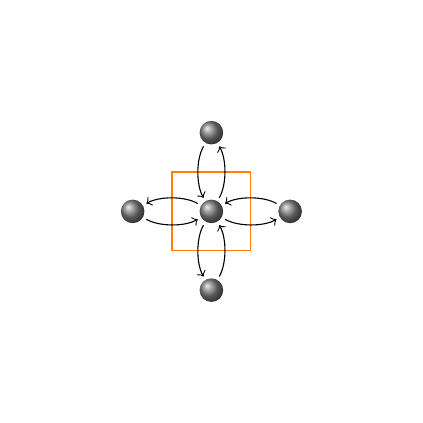
\begin{tikzpicture}[baseline, shorten >=2mm, shorten <=2mm]
    \useasboundingbox (-7/3, -7/3) rectangle (7/3, 7/3);

    \foreach \point in {(0, 0), (-1, 0), (1, 0), (0, -1), (0, 1)} {
        \shade [ball color=gray] \point circle (1.5mm);
        }

    \draw [orange] (-0.5, -0.5) rectangle (0.5, 0.5);

    \foreach \point in {(-1, 0), (1, 0), (0, -1), (0, 1)} {
        \draw [<-] \point to [bend left]  (0, 0);
        \draw [->] \point to [bend right] (0, 0);
        }
\end{tikzpicture}
